\chapter{Experimental Validation and Performance Evaluation}
\label{chap:evaluation}

This chapter details the empirical test methodology and benchmark findings across four representative operational scenarios.

\section{Measurement Setup and Methodology}
Benchmarking was conducted by dispatching concurrent bursts of 100 requests ($N=10$ independent repetitions) using asynchronous client runners (\texttt{load-test/attack\_simulation.py} and \texttt{load-test/protected\_run.py}):
\begin{itemize}
    \item \textbf{Scenario A (Baseline Unprotected)}: 100 requests routed directly to AI Server port \texttt{5001}.
    \item \textbf{Scenario B (Guest Traffic via Perimeter)}: 100 requests sent to Nginx port \texttt{8080} with guest credentials.
    \item \textbf{Scenario C (Employee Quota)}: Evaluates employee quota limits (60 req/min) via the Gateway.
    \item \textbf{Scenario D (Admin Role)}: Evaluates privileged administrators bypassing rate limit restrictions.
\end{itemize}

\section{CPU Peak Utilization Analysis}
As illustrated in Figure~\ref{fig:benchmark_cpu}, the unprotected backend experiences immediate computational saturation, reaching a peak CPU utilization of \textbf{98.5\%}. Under Scenario B, the multi-tier defense architecture drops \textbf{95\%} of non-compliant requests at the perimeter, maintaining backend CPU utilization at an optimal \textbf{10.0\%}.

\begin{figure}[htbp]
\centering
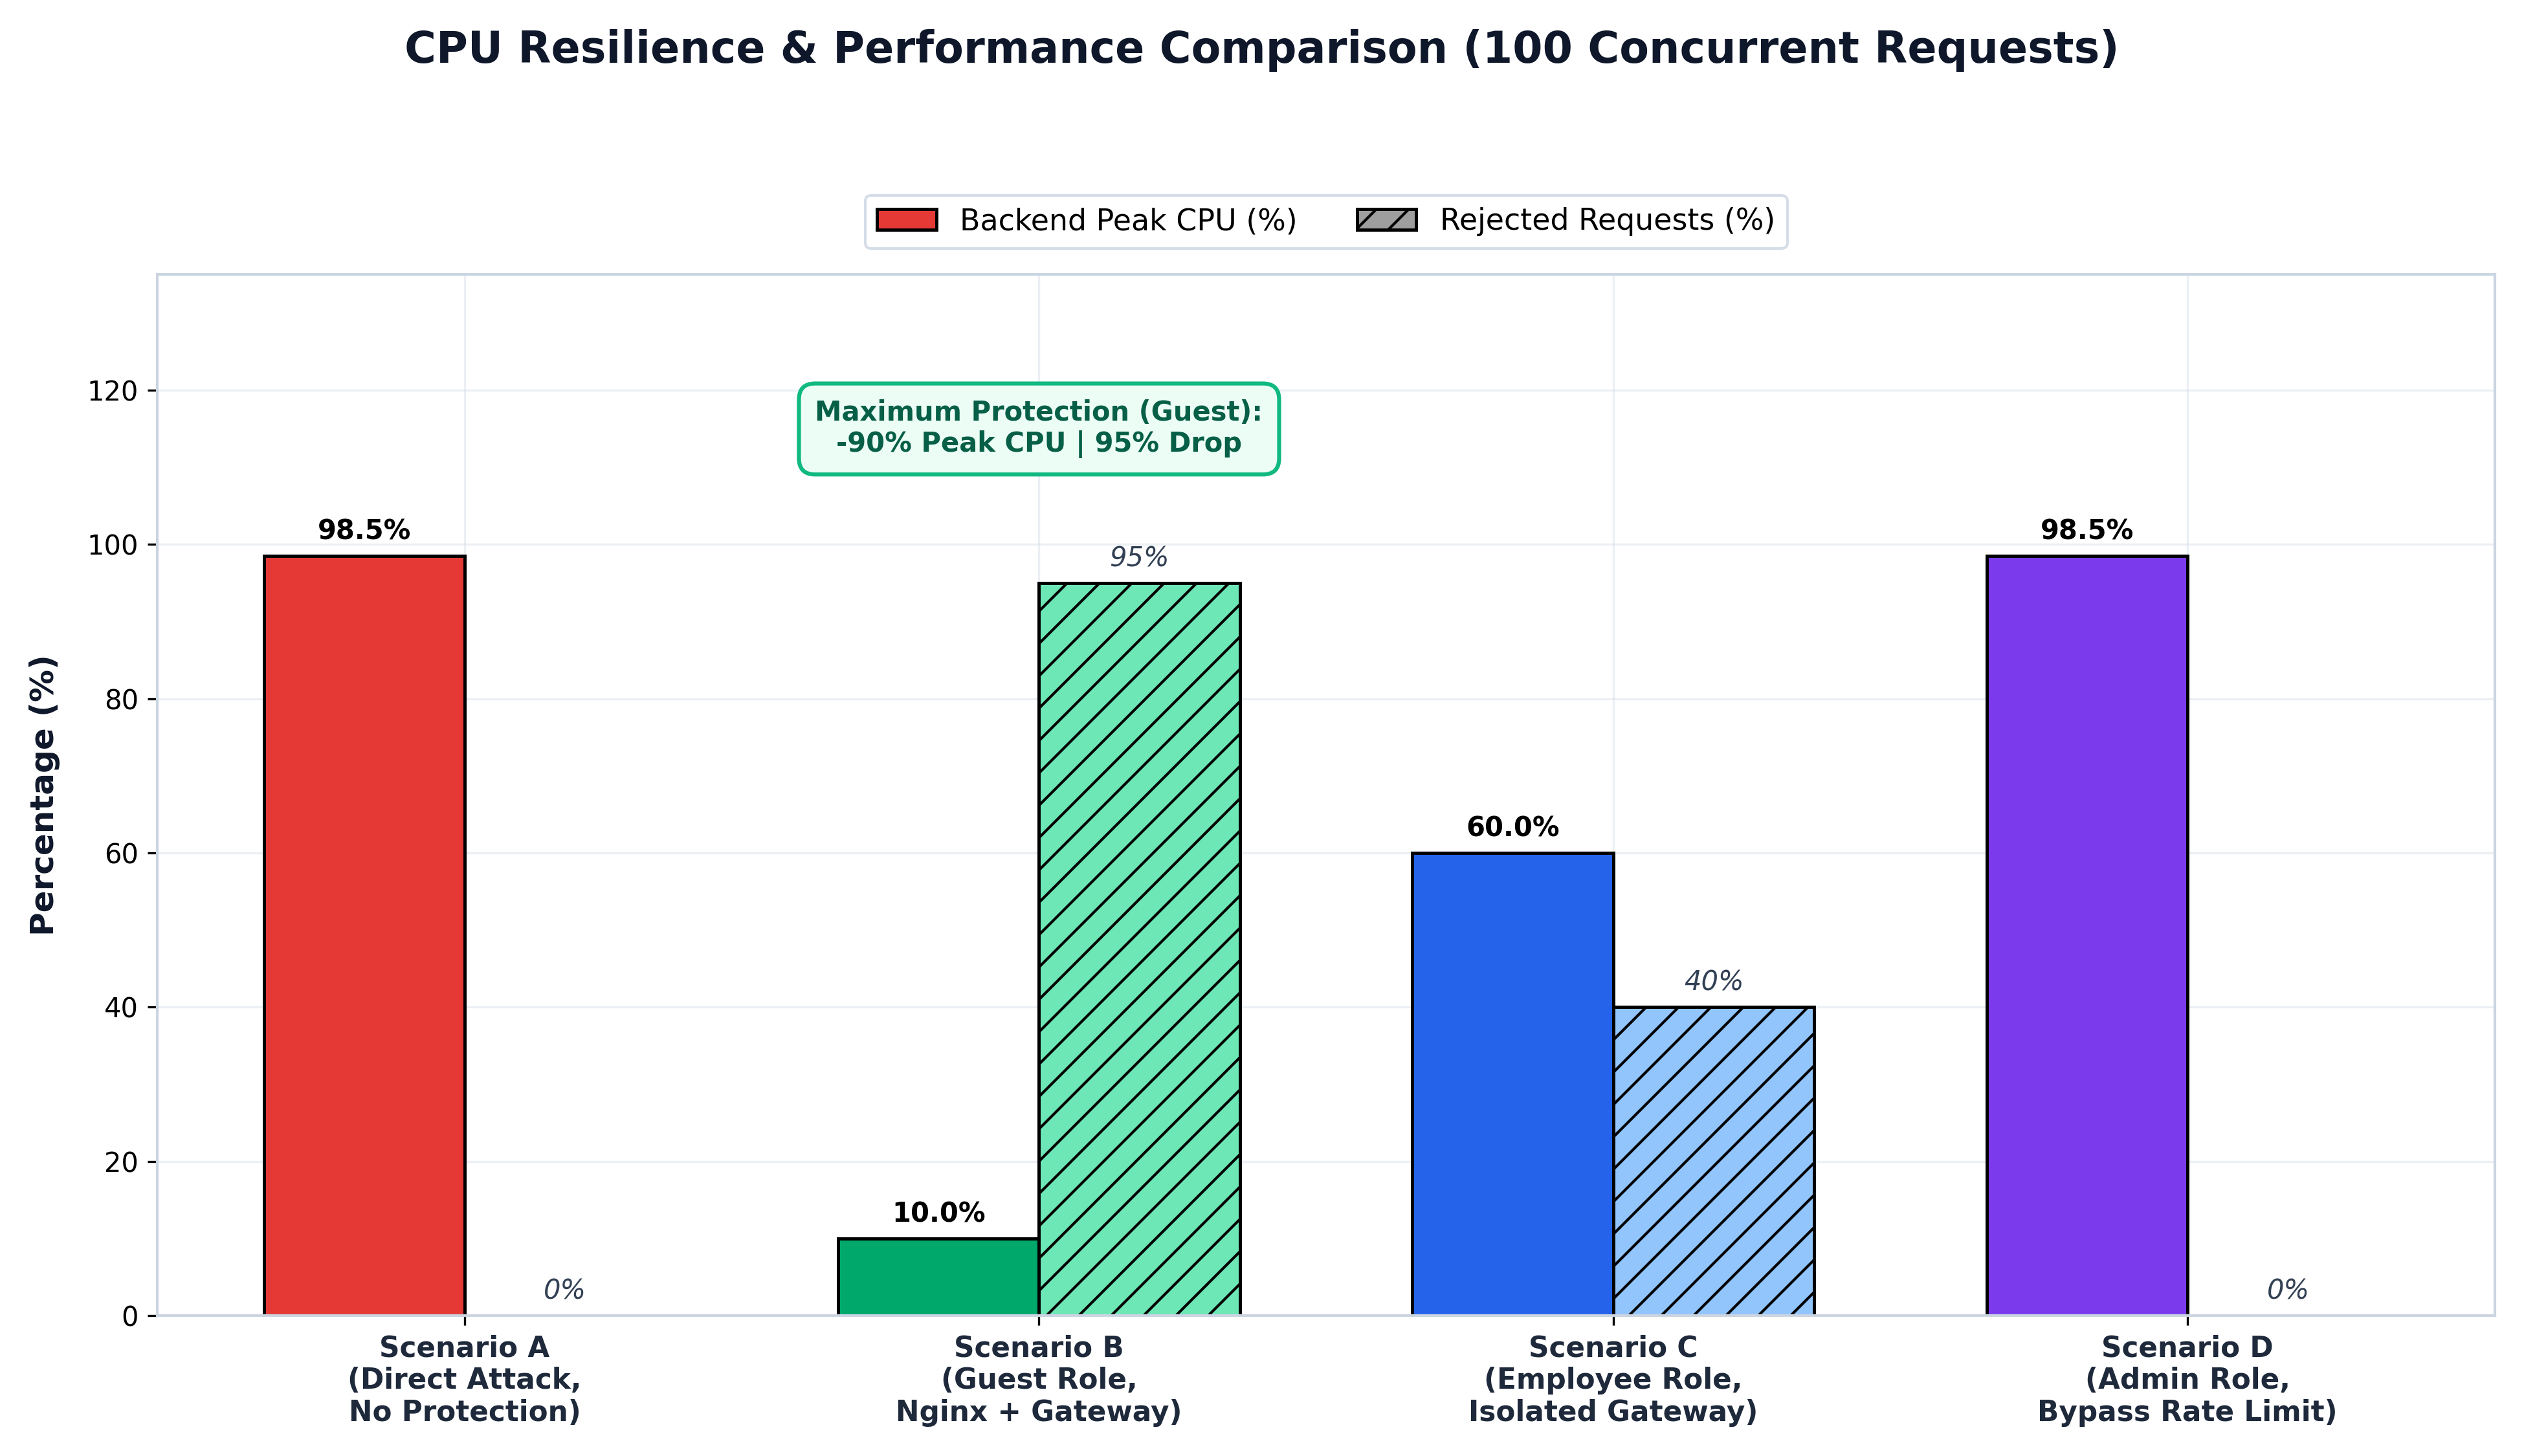
\includegraphics[width=0.92\textwidth]{figures/benchmark_cpu_peak.png}
\caption{Backend CPU Peak Resilience and Dropped Request Ratio Across Scenarios.}
\label{fig:benchmark_cpu}
\end{figure}

\section{Latency Efficiency: Backend Processing vs. Perimeter Drop}
Figure~\ref{fig:benchmark_latency} highlights the orders-of-magnitude efficiency achieved by early rejection:
\begin{itemize}
    \item \textbf{Accepted AI Inference}: Average execution time of $\approx 2000.0\,\text{ms}$ ($\sim 2.0\,\text{s}$).
    \item \textbf{Perimeter Volumetric Drop (Nginx)}: Dropped in \textbf{1.8 ms} via \texttt{HTTP 429}.
    \item \textbf{Gateway Policy Drop (RBAC / IDS)}: Dropped in \textbf{3.5 ms} via \texttt{HTTP 429/400}.
\end{itemize}

\begin{figure}[htbp]
\centering
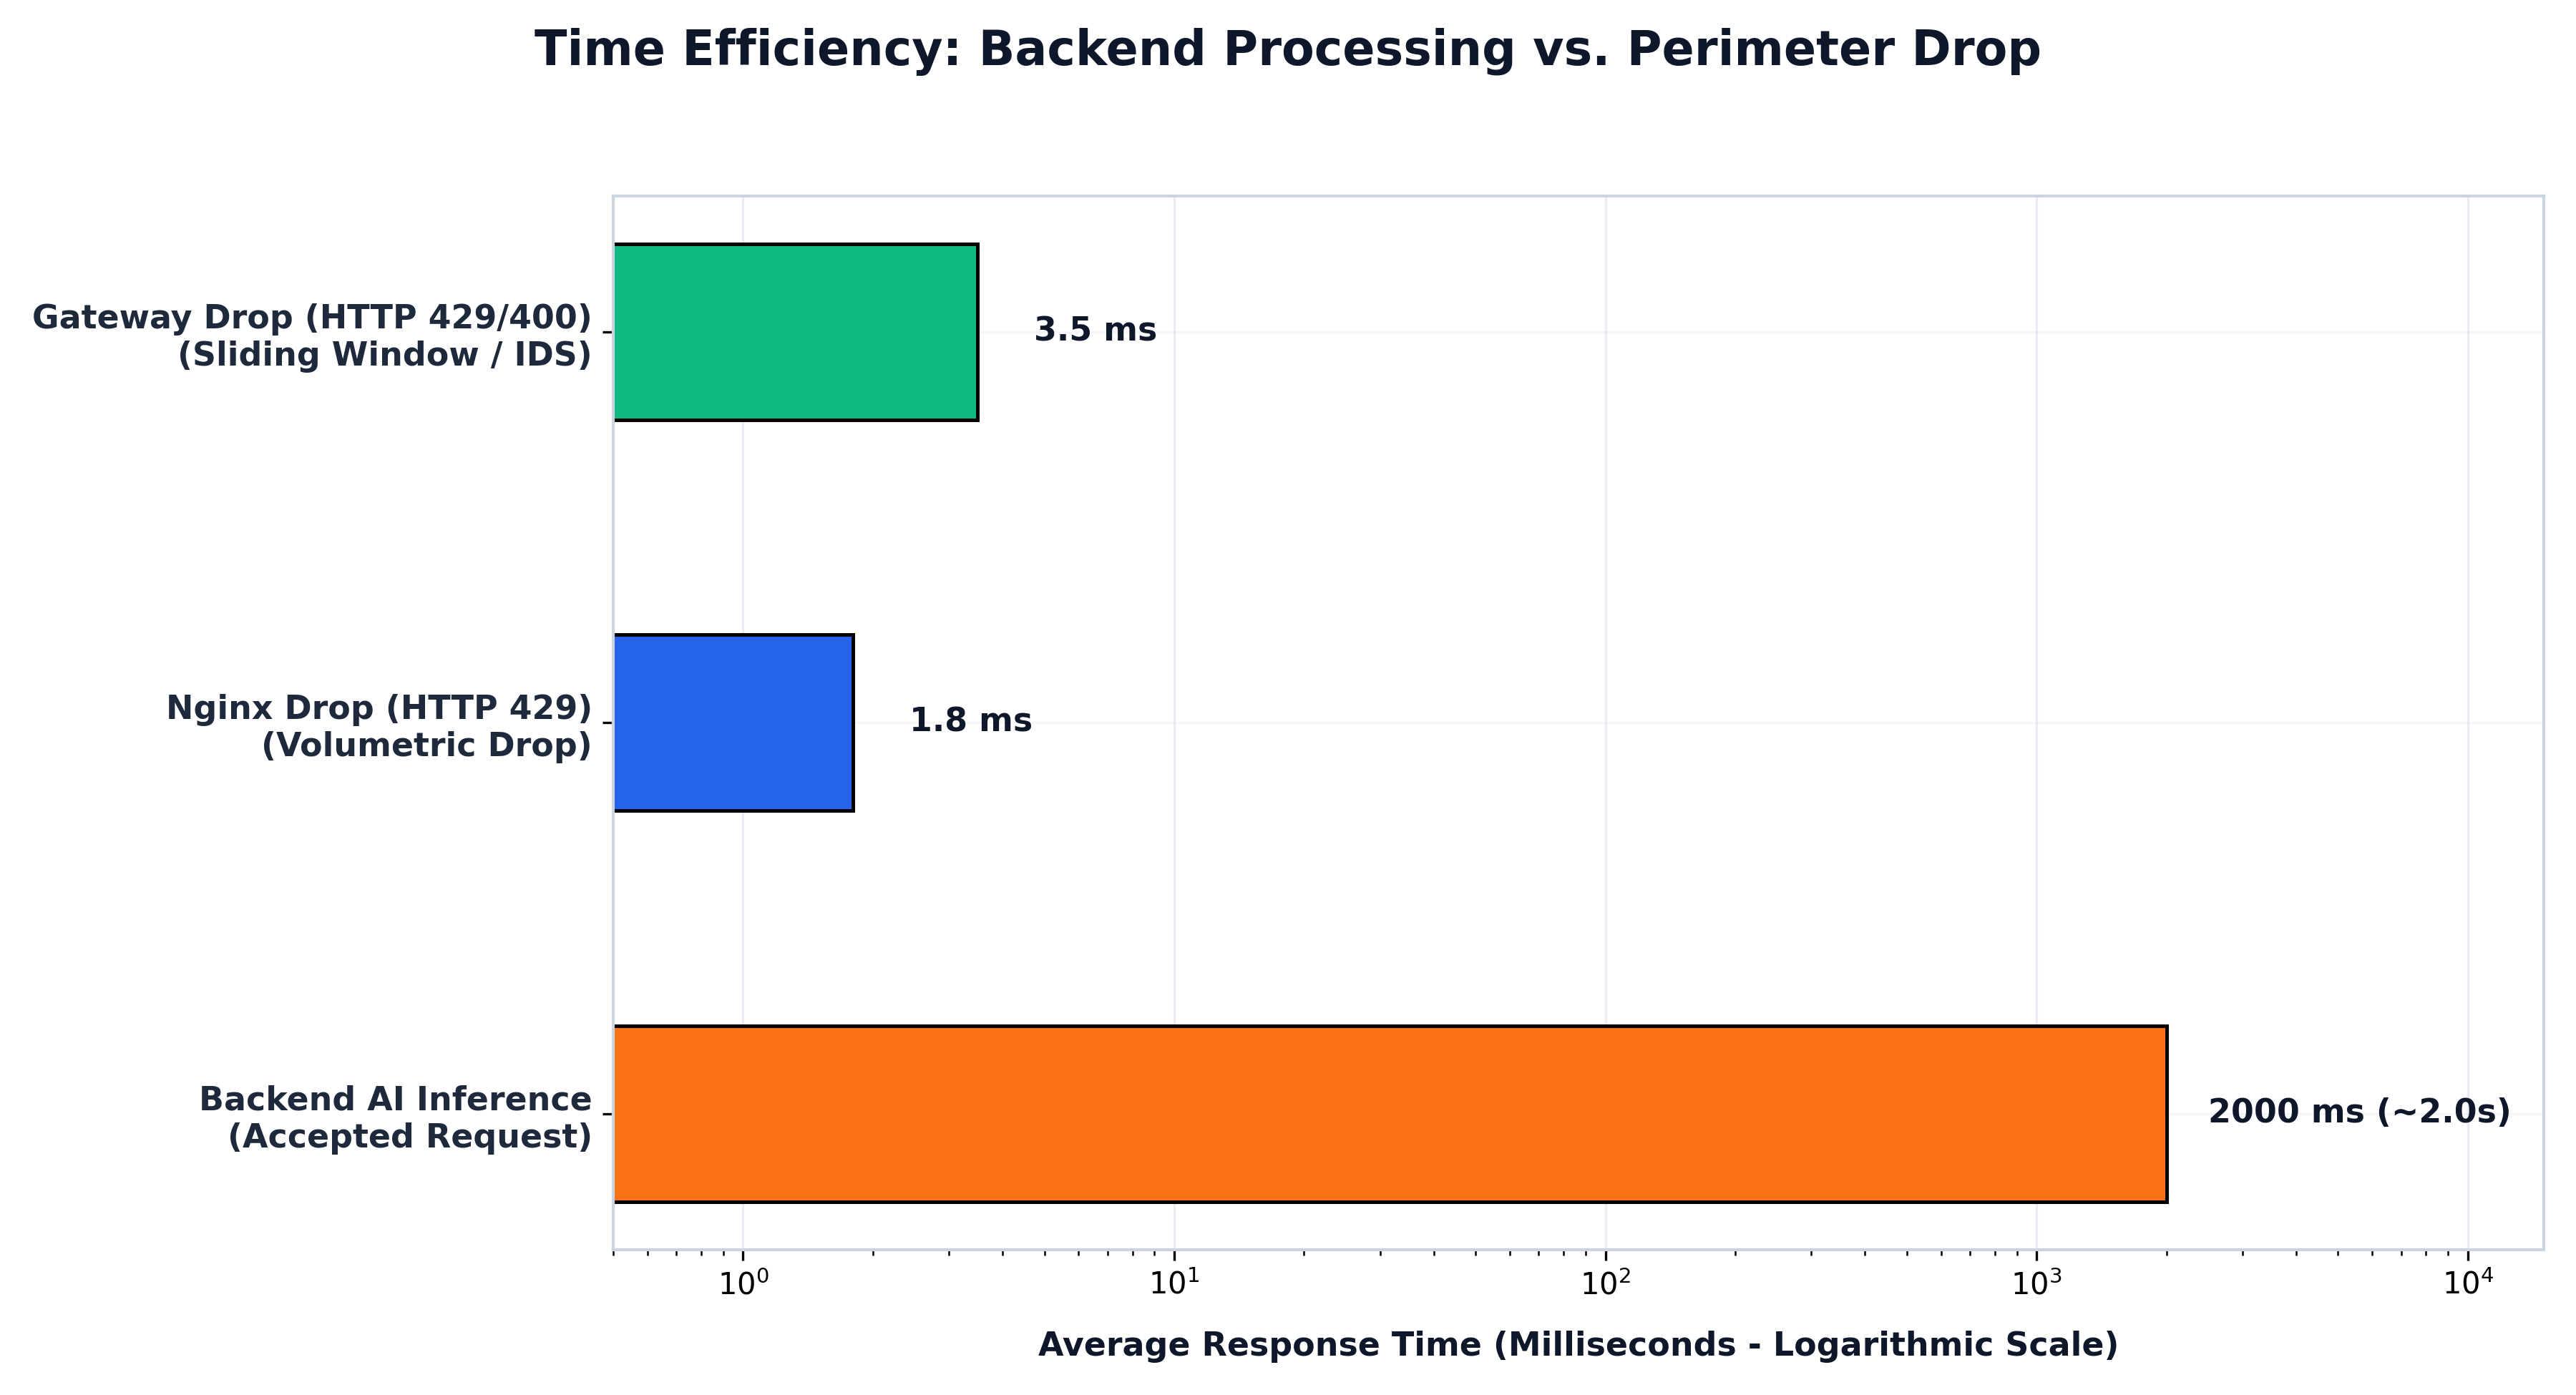
\includegraphics[width=0.90\textwidth]{figures/benchmark_latency_time.png}
\caption{Response Latency Comparison (Logarithmic Scale): Backend Inference vs. Tier Drops.}
\label{fig:benchmark_latency}
\end{figure}

Rejecting unauthorized traffic in under 4ms preserves computational throughput and guarantees service availability for legitimate users.
